\documentclass[12pt]{article}
\usepackage{epic,latexsym,amssymb}
\usepackage{color}
\usepackage{tikz}
\usepackage{geometry,graphicx,verbatim,amsmath}
\usepackage{tikz,ifthen}
\usetikzlibrary{calc}

\begin{document}

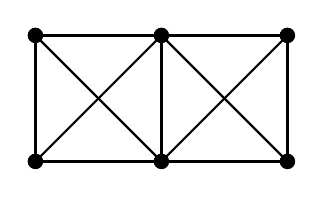
\begin{tikzpicture}[scale=0.8,style=thick]
\tikzstyle{every node}=[draw=none,fill=none]
\def\vr{3pt} 
%% vertices defined %%
\path (0,0) coordinate (v1);
\path (2,0) coordinate (v2);
\path (4,0) coordinate (v3);
\path (0,2) coordinate (v4);
\path (2,2) coordinate (v5);
\path (4,2) coordinate (v6);
%% edges %%
\draw (v1) -- (v2) -- (v3) -- (v6) -- (v5) -- (v4)  -- (v1);
\draw (v1) -- (v5) -- (v3);
\draw (v4) -- (v2) -- (v6);
\draw (v5) -- (v2);
%
%% vertices %%%
\draw (v1)  [fill=black] circle (\vr);
\draw (v2)  [fill=black] circle (\vr);
\draw (v3)  [fill=black] circle (\vr);
\draw (v4)  [fill=black] circle (\vr);
\draw (v5)  [fill=black] circle (\vr);
\draw (v6)  [fill=black] circle (\vr);
%% text %%
\end{tikzpicture}

\end{document}